%!TEX root = ../thesis.tex
%*******************************************************************************
%*********************************** First Chapter *****************************
%*******************************************************************************

\chapter{Herramientas BPM y Detección de Fallas}  %Title of the First Chapter

\ifpdf
    \graphicspath{{Chapter1/Figs/Raster/}{Chapter1/Figs/PDF/}{Chapter1/Figs/}}
\else
    \graphicspath{{Chapter1/Figs/Vector/}{Chapter1/Figs/}}
\fi

Los procesos de negocio se vieron fuertemente influenciados con el surgimiento de la computación y la comunicación digital, pues con este desarrollo tecnológico fue posible contar con herramientas capaces de automatizar en gran medida los procesos de negocio exitentes. Una de las principales funcionalidades de estas herramientas, es que los procesos de negocio se pueden definir como un flujo de trabajo o workflow, lo que permite que abstraer los procesos de negocio e implementarlos sea más fácil y eficiente. En principio surgieron los sistemas WFM (Workflow Management Systems), los cuales permiten automatizar multiples tareas relaciondas con los proceoss de negocio. Sin embargo, los sistemas WFM no permiten controlar los procesos de negocio eficientemente, por lo cual se desarrollaron los sistemas BPM (Business Process Management Systems). Estos no solo permiten automatizar la ejecución de los procesos de negocio, si no que también se enfocan en la gestión de las operaciones, la organización del trabajo, y buscan que los prceosos de negocio sean más eficientes [55, 56]. Por muchos años se ha venido trabajando con sistemas BPM, y se han abordado problematicas relaciondas con la definición de los procesos de negocio, los tiempos que toma gestionar dichos procesos, entre otras. Sin embargo, con el amplio uso de la inteligencia computacional surgen retomas más interesantes, como por ejemplo predecir el comportamiento de los items de trabajo de determinado proceso de negocio a partir de la información generada por los sistemas BPM. 


%********************************** %First Section  **************************************
\section{Sistemas BPM (Business Process Manager Systems)} %Section - 1.1 
\label{section1.1}

La gestión de procesos de negocio (BPM, Business Process Management) es una metodología que busca controlar, analizar y mejorar los procesos de negocio en las organizaciones mediante técnicas, métodos y herramientas de software, estas últimas son denominadas sistemas BPM o en inglés BPM systems. Antes del surgimiento de los sistemas BPM, se contaba con sistemas WFM (Workflow Management Systems), estos sistemas se enfocaban principalemnte en la automaticación de los procesos de negocios, sin embargo perdian de vista aspectos relevantes relacionados con el control y mejoramiento de los procesos de negocio. Es por esto que surgen los sistemas BPM, los cuales también permiten obtener múltiples abstracciones de los procesos de negocio mediante la definición de flujos de trabajo o workflows \cite{VanderAalst2004}, en estos flujos de trabajo se defienen los pasos que se deben seguir en la gestión del procesos de negocio, también se definen las decisiones que se deben tomar dentro del proceso a partir de la información dada. Cada instancia de estos workflows se denomina un ítem de trabajo o workitem, y se encargan de ejecutar los pasos del proceso definido en la herramienta BPM teniendo encuenta información especifica, generalmente esta asociada una petifción, solicitud, requerimiento, etc. Es común que para cada uno de estos workitem se registre un gran número de sucesos de eventos o event logs, estos corresponden a los pasos o eventos que ha tenido o ejecutado cada uno de los workitems. Estos event logs pueden ser almacenados en diferentes maneras, como por ejemplo una base de datos, o archivos planos. 

En los sistemas WFM y BPM la concurrencia es un aspecto muy importante, dado que generalmente en los procesos de negocio actuales es usual que se cuente con un alto número de workitems activos al mismo tiempo, y tambien es usual la ejecución de varias tareas en paralelo. Otro aspecto importante es la tolerancia a fallas, dado que en un proceso de negocio la operación es un aspecto critico, lo que hace necesario contar con sistemas robustos. Partiocularmente los sistemas BPM, se enfocan principalmente en la información relacionda con el negocio, con el fin de identificar tendencias o comoprtamientos dentro del procesos de negocio, y asi poder tomar decisiones en tiempo real, y igual que tener control dentro del procesos [56]. Todo lo anterior es bastante relevante, sin embargo, los procesos de negocio actuales son más complejos, y dependen en gran medida de los sistemas de información, con lo cual es necesario contar con estrategias mas sofisticadas al momento de intentar describir los procesos de negocio, y entender y predecir su comportamiento, es por esto que surge la minería de proceosos.

La metodología BPM propone un proceso ciclico para la implementación de los proceoso de negocio organizacionales y su constante mejoramiento. Este ciclo de vida comprende cuatro fases, el diseño del proceso (Process desing), la configuración del sistemas (System configuration), promulgación del proceso (Process enactment) y diagnóstico (Diagnosis) [1]. 


\begin{figure}[htbp!] 
\centering    
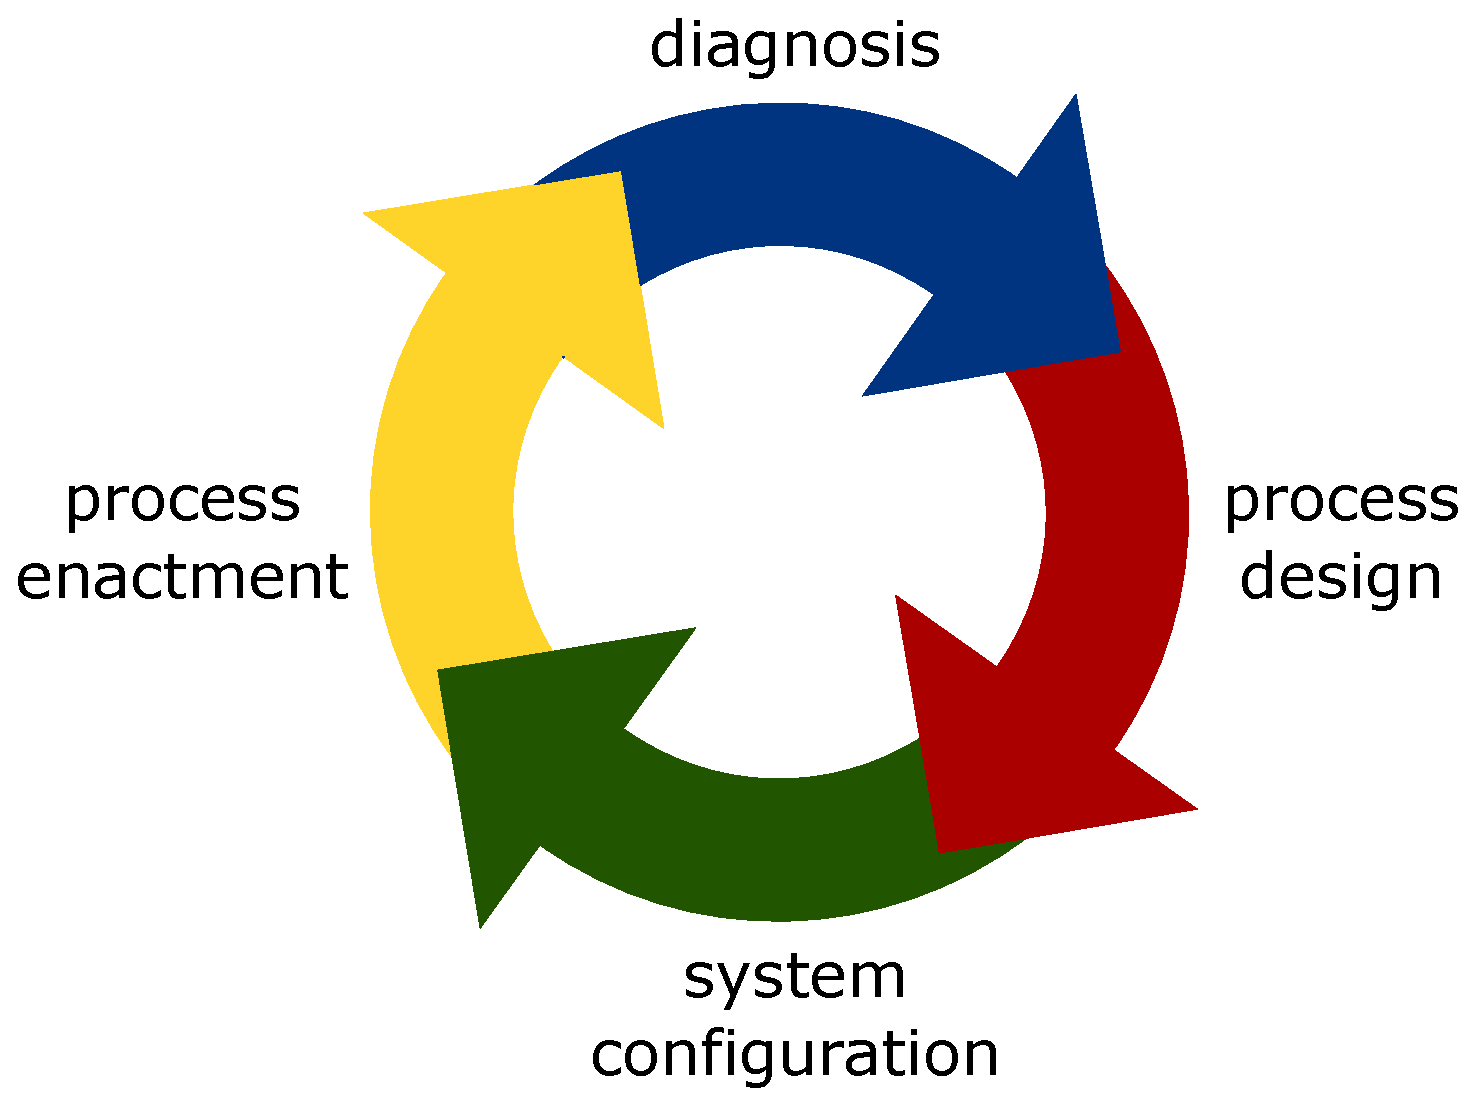
\includegraphics[width=0.5\textwidth]{Chapter1/Figs/Figure_lifecycle}
\caption[CicloVida]{Ciclo de vida del proceso de BPM}
\label{fig:CicloVida}
\end{figure}



Los procesos de negocio varian su comportamiento contantemente en el tiempo, por la cual la metodología BPM propone o define esta fase de diseño o rediseño del proceso, este rediseño no necesariamente involucra una nueva configuración del sistema, por ejmplo: simplementa podría consistir en modificar el comportamiento como es operado el proceso. Luego de realizar todo el analísis del rediseño dele proceos, se continua con la fase de configuración del sistema, la cual consiste en realizar las parametrizaciones que sean necesarias en la herramienta BPM, las herramientas BPM en generas estan contruidas de tal manera que no sea necesario realizar desarrollo de nuevo código, sin embargo existiran excepciones. La fase de promulgación del proceso es la siguiente, en esta fase todoas las configuraciones realizadas en la fase anterior son usadas de manera productiva. Finalmente, en la fase de diagnostico, se analizan los cambios presentados a lo largo dele tiempo, al igual que los aspectos de mejora que pueden ser aplciados en el procesos, de tal manera que en fase de deseño se inicie nuevamente el cliclo. LA siguiente grafica ilustra el proceso:


En la actualidad existe una institución que se encarga de describir como deben funcionar o como deben ser construidos los sistemas WFM o BPM, esta se llama Workflow Management Coalition (WfMC), fundada en 1993 [55], esta propone un esquema de arquitectura sugerido para las herramientas de este tipo. Algunos de los compoenentes mas relevantes son por ejemplo el workflow enactment serevice, este provee un ambiente de ejecución que permite controlar y ejecutar los diferentes workflow activos, y se podría componer de uno o mas workflow. engines. estos ultimos admnistran parte de los worflows y partes de los recursos [55]. También otro componente con el que se cuenta, son las herramientas de definición dle proceso, 


El core de WFM/BPM es workflow enactment service. -> compuesto por workflow engines
El principal componente de los sistemas BPM/WFM es el llamado workflow enactment service, este provee un el entorno de ejecución adecuado para la ejecución de los workflows en el sistema, este servicio puede contar o hacer uso de multiples workflow engines [55]. 

Las herramientas de definición de procesos (process definition tools), estas herramientas permiten realizar el diseño del proceso, generalmente usando notación para el modelado. Tambien permiten realizar analisis de los procesos y simular los flujos definidos [55]. 


Los usuario finales se counican con los workflows systems por medio de los workflow client applacations. Generalmente por los denominados in-baskets, en estos baskets son presentandos los workitems al usuario final, de tal manera que sobre los workitems se puedan ejecutar tareas especificas. 

Como todo sistema BPM se espera poder controlar el proceso, por dicha razon se tienen los administration and monitoring tools, estas herramientas se encangar de registrar el proceso de los casos, al ogual que detectar cuaellos de bottela, entre otras tareas. 

Estos componentes se pueden visualizar en la siguiente figura [55]


EN la siguiente figura (Figura 21 [55]) referencia [1], se puede visualizar un poco mas en detalle los disferentes compoentes de los sistemas bpm, al igual que los conjuntos de datos que se manejan y su interacción con los diferentes usuarios. Nuevamente en este esquema se puede evidenciar que el Enactment service es el core de los sistemas bpm, e interactua directamente con los demas compoenentes [55].

Arquitectura como las Service Oriented Computing, o la Service Oriented Architecture, han tenido un gran impacto sobre los sistemas BPM/WFM, permitiendo que los componentes sean más desacoblados y dando mas flexibilidad a las herramientas, dado que ciertos trabajos se pueden tercedizar o usar desde otroso compoentens, faciliando la integarción con otros sistemas [55]. 

Finalmente, las propuestas mas resientes en arquitectura, son las plateadas en la nube, las cuales comprenden un esquema SaaS, PaaS, o IaaS. 



%********************************** %Second Section  **************************************
\section{Detección de Fallas en sistemas BPM} %Section - 1.2
\label{section1.2}

Los sistemas BPM debe lidiar constantemente con un gran numero de casos o work items activos, al igual que con un numero significativo de usuarios concurrentes.Tambien debe comportarse adecuadamente frente a los cuellos de botella, y responder rapidamente a las peticiones que le son realidadas. Algo que no ayuda mucho es los grandes volumenes de informaicón que debe almacenar. Adicional a esto, generalmente ocurre que los procesos de negocio no sean modelados de acuerdo a la realidad, o que cambine con el tiempo. Es por esto que la metodología BPM propone un proceso de implementación ciclico, donde constantemente se esta recalibrando el proceso implementando, al igual que se realizan ajustes en la plataformar, como mejoramiento en el desempeño de las bases de datos, o en la plataforma misma, como por ejemplo un mejoramiento de las caracteristicas fisicas donde esta desplegado el sistema. 

Adicional a esto, las arqutiecturas propuestas por compoentnes, como las mencionadas anteriormente, (SOC o SOA), permite desacoplar los sistemas de un solo core, de tal manera que la afectación al servicio no sea tan traumatica, y tambien dando flexibilidad a la implementación de las soluciones. Sin emgargo, con los volumenes de información tan altos, y la cantidad de workitems activos, se hace evidente que estos controles no son suficientes para afrontar las fallas, dado que puede ocurrir que el sistema presente intermitencias, y afecto solo una pequeña parte de los workitems activos, lo que no permitiria que fueran visibles, pero que si podria generar un impacto negativo en el proceso, 



Dado estos nuevos retos en los sistemas BPM, es necesario pensar en la mineríaa de procesos.










%********************************** %Third Section  **************************************
\section{Minería de Procesos para la detección de fallas en sistemas BPM} %Section - 1.3
\label{section1.3}

En las organizaciones actuales, diseñar u obtener modelos de los diferentes procesos de negocio puede llegar a ser una tarea compleja, ambigua, que toma mucho tiempo y que requiere de un conocimiento profundo del negocio. La minería de procesos busca resolver estas dificultades haciendo uso de los sucesos de eventos, dado que estos contienen información detallada que permite llevar trazabilidad de cada una de las tareas ejecutadas por los procesos de negocio. Estos sucesos de eventos se registran como una secuencia de datos que generalmente contienen información del tipo de actividades u operaciones ejecutadas por cada ítem de trabajo, al igual que del tiempo de ocurrencia de estos eventos; vale la pena resaltar que estos sucesos de eventos no siempre se almacenan de una manera estructura. Las herramientas BPM juegan un rol importante en este ámbito, pues buscan apoyar los procesos de negocio a partir de la definición de flujos de trabajo o workflows.

En este sentido, en [1] se plantea un completo manual sobre minería de procesos en el cual se analizan los diferentes patrones que pueden presentarse en los workflows, también se exponen problemas típicos de semántica que limitan el uso de la tecnología BPM o WfMS (En inglés Workflow Management Systems). En este trabajo resalta la importancia de los sistemas BPM debido a que se han convertido en una potente herramienta para la automatización de los procesos, prueba de ello es la gran cantidad de sistemas que han surgido a lo largo del tiempo.

Muchos de los trabajos realizados hasta el momento aplican técnicas de minería de procesos sobre workflows simulados, donde los datos analizados corresponden a datos de pruebas. Sin embargo en [3] por ejemplo se aplica la minería de procesos en el mundo real, donde se tiene en cuenta la información registrada por un sistema WFM, este sistema registra los sucesos de eventos necesarios para generar un modelo que permita describir el proceso; en este trabajo se puede ver que la minería de procesos no solo se aplica a sistemas de tipo WFM, sino que también se puede aplicar sobre sistemas CRM (En inglés Customer Relationship Management), ERP (En inglés Enterprise Resource Planning), entre otros, dado que estos sistemas soportan también procesos de negocio y registran sucesos de eventos.

En la actualidad existen varios trabajos en los que se abordan los retos existentes en la minería de procesos, en [22] por ejemplo se propone un algoritmo que facilita la tarea de definición de modelos de proceso a partir de sucesos de eventos; en este trabajo también se busca ampliar el uso de los sistemas que se basan en la definición de workflows, como por ejemplo los sistemas BPM. En [23] se aborda el mismo problema que en [22], pero desde el ámbito del aprendizaje automático, y haciendo uso de FWF-Net (En inglés Flexible Workflow Modeling Language), un lenguaje de modelado de workflows flexible que permite modelar y simular procesos de negocio. El algoritmo propuesto en este trabajo no solo maneja efectivamente la concurrencia en los procesos, sino que también se comporta bastante bien ante la recurrencia presentada en los mismos, este algoritmo al igual que en [22], permite transformar el resultado obtenido a una definición del workflow fácilmente. En [2] se usa la misma metodología que en [23], pero en este se propone el denominado algoritmo (alpha), el cual permite identificar nuevos modelos de proceso de negocio a partir de información de sucesos registrada por un sistema WFM, sin embargo es importante tener en cuenta que si el proceso presenta tareas ocultas, tareas duplicadas o enrutamientos complejos surgen debilidades en el algoritmo [23].

Sin embargo, a diferencia de los trabajos anteriores en los que se buscaba refinar el modelo del proceso a partir de la secuencia de eventos, en la actualidad la minería de procesos propone nuevos retos, como por ejemplo la posibilidad de predecir tiempos de completitud de las tareas o instancias de trabajo existentes [31]. En [4] se propone un método que permite predecir el futuro de una instancia de trabajo, es decir hace posible identificar el tiempo restante de ejecución de cada instancia de trabajo, o el tiempo que tomará finalizar determinada actividad. La idea básica de este trabajo es implementar un sistema de anotación de transiciones, el cual es entrenado a partir de las transacciones ejecutadas con anterioridad, con lo que es posible realizar las predicciones propuestas.

El problema de predecir la evolución de un workitem, ha llevado a la minería de procesos a usar técnicas provenientes del aprendizaje automático, específicamente técnicas que permitan modelar y clasificar secuencias de datos como las cadenas ocultas de Markov (En inglés Hidden Markov Models - HMM) [18]. Los HMM son ampliamente usados en un sinnúmero de aplicaciones de aprendizaje automático y reconocimiento de patrones, incluyendo la minería de procesos, dado que presentan buenos resultados al modelar datos secuenciales [24]. En [27] es implementado un HMM para modelar sucesos de eventos registrados por sistemas BPM o WFM. En este trabajo HMM se describe como un autómata finito donde las transiciones tienen una probabilidad asociada y los estados están asociados a un conjunto finito de salidas que cuentan con cierta probabilidad. HMM se ajusta bastante bien a los datos debido a que los procesos de negocio generalmente se pueden entender como un proceso de Markov en el cual existe una transición entre estados. En [12] se aborda el problema de la minería de procesos usando HMM como un marco de trabajo básico para un algoritmo de clasificación de secuencias, en este trabajo se evidencia un aporte significativo por parte de HMM a algoritmos de clasificación de secuencias al permitir identificar actividades paralelas, ciclos en el proceso, entre otros patrones típicos en los procesos de negocio. Teniendo en cuenta las capacidades de modelado expuestas, en [5] se aborda el mismo problema que en [4], pero haciendo uso de HMM. Se compara HMM con otros modelos estadísticos, sin embargo los autores concluyen que HMM provee mejores resultados en tareas predictivas.

Aunque los HMM han logrado buenos resultados en muchas aplicaciones, existe un problema debido a que las secuencias de datos no siempre cuentan con una distribución de tiempo constante, tal como lo supone HMM. En [28] se abarca el problema de reconocimiento de patrones sobre datos de series de tiempo en señales de onda, sin embargo debido a las debilidades presentadas por HMM al manipular datos con tiempo variable se propone una extensión de HMM, denominada HSMM (En inglés Hidden Semi-Markov Model). Este modelo elimina las distribuciones constantes o geométricas de los tiempos de duración de cada uno de los estados del proceso que generalmente son asumidas en HMM [8]. Al igual que los HMM, los HSMM han sido usados en diferentes tareas de reconocimiento de patrones [6,32], incluyendo también la minería de procesos [17]. En [17] se usa un modelo HSMM para modelar secuencias de eventos en un problema de predicción de fallas, precisamente por la capacidad de este modelo de incluir la información temporal explícita y la importancia que dicha información tiene para el problema de detección abordado. El enfoque de este trabajo es hacia la eficiencia en el procesamiento de los datos, ya que el modelo HSMM es computacionalmente mucho más costoso que el modelo HMM estándar. La solución propuesta es a nivel de hardware, permitiendo un entrenamiento mucho más rápido del modelo, pero limitando su aplicación en otros contextos ya que la solución planteada es muy específica. De manera similar, en [9] se propone el uso de HSMM para la predicción de fallas en un sistema de telecomunicaciones comercial, donde se analizan los sucesos de eventos registrados en el sistema, y se reconocen ciertos patrones de comportamiento que indican si se puede generar una falla inminente. Por otro lado, en [32] se aborda el tema de detección de intrusiones anormales en un sistema, por medio de reconocimiento de patrones usando HSMM. Para identificar dichos patrones, el modelo toma en cuenta los sucesos de eventos registrados por el sistema. Los resultados experimentales muestran que la detección de fallos depende de la longitud de la secuencia de eventos, alcanzando niveles de predicción entre el 93 y el 100 porciento, lo que permite reforzar la idea de que usar modelos HSMM en el monitoreo de sistemas en línea, puede ser un alternativa viable.

Con el objetivo de refinar y aumentar la capacidad de modelado de los HSMM, en [16] se presenta un nuevo modelo denominado NHSMM (En inglés Non-stationary Hidden Semi-Markov Model), el cual además de incorporar la información temporal de las secuencias, afina la probabilidad de transición de los estados incluyendo la dependencia del tiempo. En NHSMM se define una distribución de probabilidad de transición que permite reflejar la propiedad no estacionaria de los procesos de Markov convencionales. Al asignar una probabilidad al tiempo que dura el proceso en determinado estado, se establece que diferentes duraciones en un estado afectan la elección del nuevo estado al que se va a transitar. NHSMM no solo tiene en cuenta la duración explícita en un estado, sino que también selecciona a donde se hará la transición de acuerdo con dicha duración. Sin embargo, NHSMM no ha sido ampliamente usado, debido principalmente al costo computacional que implica su entrenamiento.

Otras técnicas de aprendizaje automático como las redes neuronales artificiales también han sido exploradas en el contexto de la minería de procesos, sin embargo estas no han alcanzado el mismo interés que los modelos antes mencionados. En [52] se hace una revisión completa de las investigaciones realizadas sobre la minería de procesos por un periodo de once años, de todos los trabajos analizados menos del dos por ciento corresponde a investigaciones que involucran las redes neuronales artificiales. En [53] se realiza un estudio exploratorio en el uso de las redes neuronales artificiales en la extracción de conocimiento a partir de procesos no estructurados, en este trabajo se evidencia que uno de los principales problemas al usar redes neuronales artificiales en la minería de procesos es la alta dimensionalidad, al igual que la pérdida semántica en la información, dado que se puede llegar a obtener un modelo que no representa el proceso analizado.

El algoritmo de entrenamiento de los HMM, conocido como Baum-Welch (o Forward-Backward), es una implementación dinámica del algoritmo de Esperanza y Maximización (EM), el cual a su vez corresponde a una implementación del criterio de máxima verosimilitud. Generalmente EM produce buenos resultados, aunque puede sufrir de problemas de sobreajuste y puede tomar mucho tiempo en converger, particularmente para datos con una dimensionalidad alta [26]. Para un HMM estándar, con secuencias de longitud T y con N estados ocultos, la complejidad en términos de memoria del algoritmo BW crece linealmente con T y N, obteniendo una complejidad del orden O(N T ) , mientras que la complejidad respecto al tiempo crece cuadráticamente con N y linealmente con T, lo que implica una complejidad del orden de O (N 2 T ) . Estas medidas se ven fuertemente afectadas para los modelos dependientes del tiempo [9]. En una implementación sencilla de HSMM la complejidad en términos de memoria es igual a la de un HMM estándar, sin embargo la complejidad computacional durante el entrenamiento es del orden de O((N 2 + N D 2 )T ) , donde D es la máxima cantidad de tiempo que se permanece en un estado [15]. Finalmente en un NHSMM la complejidad computacional del entrenamiento es del orden de O (N 2 T D 2 ) [16].

Teniendo en cuenta la complejidad computacional de los modelos HMM y sus modificaciones, el uso de dichos modelos para resolución de problemas en el mundo real se ve limitado a la cantidad de información que es necesario procesar. Por dicha razón se han propuesto algunas alternativas que intentan reducir la complejidad computacional de los algoritmos de entrenamiento [14,31]. Otras propuestas intentan abordar dicho problema de manera paralela y/o distribuida, ya sea modificando los algoritmos de entrenamiento [47,48], o haciendo uso de herramientas especializadas en el procesamiento de información por medio de sistemas distribuidos [30]. También existen propuestas que incluyen la implementación de componentes de hardware [17,43].

Una novedosa técnica de procesamiento paralelo, y que ha tenido una gran acogida es MapReduce. Esta técnica fue desarrollada por Google, y es orientada particularmente a los problemas que involucran el procesamiento de grandes cantidades de datos [25]. Los modelos HMM pueden ser implementados bajo el paradigma de MapReduce, sinembargo es necesario ajustar los modelos a este paradigma. Por ejemplo, en [29] se muestra la aplicación de MapReduce en HSMM, donde la implementación de este modelo es realizada sobre Spark, una plataforma ampliamente usada en el contexto de Big Data.

Para el caso de los modelos NHSMM, al momento en que se realiza esta revisión, no se encuentran alternativas publicadas para la reducción de los tiempos de entrenamiento, razón por la cual aunque su capacidad de modelado es mayor que la de los modelos HMM y HSMM, como se indicó anteriormente, su uso en el contexto de la minería de procesos aún no ha sido explorado.

%********************************** %Fifth Section  **************************************
\section{Discusión} %Section - 1.4
\label{section1.4}

